%%%%%%%%%%%%%%%%%
%% BASIC SETUP %%
%%%%%%%%%%%%%%%%%
\documentclass[12pt]{article}
\usepackage[style=apa]{biblatex}
\addbibresource{references.bib}

% Necessary packages
\usepackage{titling}
\usepackage{geometry}
\usepackage{mathptmx}
\usepackage{hyperref}
\usepackage{booktabs}
\usepackage{float}
\usepackage{graphicx}
\usepackage{titlesec}
\usepackage{setspace}
\usepackage{lscape}
\usepackage[tableposition=top]{caption}
\usepackage{indentfirst}

% Title page margins
\newgeometry{top=2in, bottom=1in, left=1.5in, right=1.5in}

% Define commands to switch margins
\newcommand{\titlepagegeometry}{\newgeometry{top=2in, bottom=1in, left=1.5in, right=1.5in}}
\newcommand{\documentgeometry}{\newgeometry{top=1in, bottom=1in, left=1in, right=1in}}

% Table of contents formatting
\setcounter{secnumdepth}{3}

% General caption setup
\captionsetup{width=1\textwidth}

% Custom label format for figures
\DeclareCaptionLabelFormat{bold}{\textbf{#1~#2}}

% Figure caption setup
\captionsetup[figure]{
  format=plain, 
  justification=centering,
  labelformat=bold,  
  labelsep=period
}

% Table caption setup
\captionsetup[table]{
  labelfont=bf,
  labelsep=period,
  position=top,
}

% Adjust spacing
\setlength{\parskip}{1.5em}
\titlespacing*{\section}{0pt}{*0}{*0}
\titlespacing*{\subsection}{0pt}{*0}{*0}
\titlespacing*{\subsubsection}{0pt}{*0}{*0}

\begin{document}


%%%%%%%%%%%%%%%%%
%% TITLE PAGE %%
%%%%%%%%%%%%%%%%%
\begin{titlepage}
    \centering
    \vspace*{-3cm}
    
\includegraphics[width=0.5\textwidth]{reports/unc-logo.png}\par
    \vspace{0.5cm}
    {\Huge\bfseries Investigating Reasons for Uninsurance in the 2023 U.S. National Health Interview Survey \par}
    \vspace{2cm}
    {\LARGE Julia G. Muller\par}
    {\Large Gillings School of Global Public Health \par}
    {\Large University of North Carolina at Chapel Hill \par}
    \vspace{3cm}
    {\large A final capstone submitted for the Master of Public Health in Applied Epidemiology \par}
    \vspace{1cm}
    {\large 15 April 2025\par}
    \vspace{1cm}
\end{titlepage}


%%%%%%%%%%%%%%%%%%%%%%%
%% TABLE OF CONTENTS %%
%%%%%%%%%%%%%%%%%%%%%%%
\newpage
\documentgeometry
\tableofcontents


%%%%%%%%%%%%%%%%%%
%% INTRODUCTION %%
%%%%%%%%%%%%%%%%%%
\newpage
\section{Introduction}

  Although the United States spends twice as much per capita on healthcare as the median industrialized nation, millions of Americans still lack insurance (Turner citation). People who do not have health insurance face increased financial strain, barriers in access to healthcare, and worse overall health outcomes (\cite{davis_uninsured_2007}). 49\% of uninsured adults report difficulty paying medical bills, compared to only 21\% of adults with private insurance (\cite{tolbert_key_2024}). Furthermore, uninsured adults are more likely to delay or forgo medical care due to cost, and face challenges accessing both preventive and specialized healthcare services (\cite{cha_reasons_2020, erly_characterization_2022}). Addressing remaining insurance gaps is critical to ensure equitable access to health care and positive health outcomes. Understanding the reasons why people remain uninsured—as well as the impact of those reasons on the length of time they go without insurance—could identify potential avenues for interventions to close the insurance gap.

While the United States has attempted to expand health coverage through expansion of the Affordable Care Act, an estimated 21.3 million adults aged 18 to 64 remained uninsured as of 2023 (\cite{tolbert_key_2024}). Various demographic factors—such as age, race, Hispanic ethnicity, income, and education level—play a role in the likelihood of being uninsured and reported reason for being uninsured (\cite{lee_convergence_2021}). Uninsurance is more prevalent among individuals who are lower income, racial minorities, Hispanic ethnicity, non-citizens, and those between the ages of 18 and 30, with these factors often intersecting (\cite{gunja_who_2019, okoro_lack_2015, wisk_inequalities_2019}). Furthermore, the reasons for not having insurance also differ across these demographic groups. In 2023, 63\% of adults aged 18 to 64 cited the high cost of insurance as their primary reason for being uninsured (\cite{tolbert_key_2024}). However, the impact of cost varies by age group; only 66.8\% of those aged 18 to 29 reported high cost as their primary reason for uninsurance, compared to 80.9\% of those aged 50 to 64 (\cite{cha_reasons_2020}). Other demographic factors, such as race and ethnicity, also influence reasons for remaining uninsured; for example, Hispanic adults were significantly more likely to report ineligibility as their primary reason for not having insurance (\cite{cha_reasons_2020}). Addressing the problem of uninsurance requires an understanding of the various reasons behind it, as well as how these reasons differ across demographic groups. Previous research has identified some of these reasons, but little has been done to explore how they correlate with the duration of being uninsured, which is a critical factor for understanding the long-term effects of uninsurance.

Relatively few studies have examined the specific reasons for uninsurance, and no studies have linked these reasons with the duration of uninsurance. Understanding this relationship is essential because the longer an individual is uninsured, the greater the risk of negative health and financial outcomes. This study aims to explore the reasons for uninsurance among adults aged 18 to 64 in the U.S. using 2023 NHIS data. By stratifying the data by demographic characteristics, this study will provide a more nuanced understanding of the barriers to obtaining insurance and the impact of these barriers on the duration of uninsurance. Ultimately, this research will inform policy recommendations aimed at closing the remaining gaps in health insurance coverage.


%%%%%%%%%%%%%
%% METHODS %%
%%%%%%%%%%%%%
\newpage
\section{Methods}

Data were obtained from the 2023 National Health Interview Survey, a nationally representative cross-sectional survey of the non-institutionalized U.S. population. All respondents were asked whether they currently had health insurance. Those who answered that they did not, were asked further questions about reasons for no insurance and duration without coverage.

Our target population is uninsured adults between the ages of 18 and 64 in the United States. These adults are not eligible for Medicare, which starts at 65 years of age. In order for individuals to be included in our study, they must be ages 18-64 and be uninsured at the time of the survey. This includes not having Medicare, Medicaid, any non-Medicaid state-sponsored health insurance program, CHAMPUS, CHAMPVA coverage, or any private insurance. Individuals who have any of these insurance plans were not included in the study. Our final study population consisted of 1,937 individuals.

Our primary exposure variable was the reasons a person does not have insurance. Uninsurance is defined as having no insurance or persons with a single service plan. The response options include: unemployment, high cost, not wanting insurance, plans not meeting needs, coverage has not started yet, missed deadline, or other reasons (not provided by the interviewer). Our primary outcome variable was time since the respondent last had health insurance, among those who were uninsured at the time of the survey. Responses were grouped by NHIS into the following categories: less than 1 year, 1 year to less than 2 years, 2 years to less than 3 years, 3 years or more, less than 5 years, 5 years or more, less than 10 years, 10 years or more, never, and unknown (refused, not ascertained, don’t know). The reasons for unknown were originally separated by NHIS, but we combined them due to small sample size. We additionally examined sociodemographic variables, including self-reported race, self-reported Hispanic, Spanish, or Latino origin or ancestry, urban or rural residence (large central metro, large fringe metro, medium- and small-metro county, or non-metro county), age in years, sex as identified by interviewer, and highest level of education completed.

For measures of occurrence, the prevalence of each reason why an individual does not have insurance was calculated in total and across covariates (race, ethnicity, urban/rural status, sex, level of education). Additionally, we calculated descriptive statistics for the duration of uninsurance, including the total average duration and average duration for each reason. 

For our analysis, we looked at the difference in the frequency distribution of reasons by different durations of time without insurance. Then, we used ANOVA to look for correlation between duration and reasons for no insurance. We used a chi-squared test to test if the difference in duration without insurance is significantly different between reasons for not having insurance. We also assessed differences in proportions across different covariate strata, including urban vs rural, race, and ethnicity. Analyses were performed in SAS and R.

For this study, our sample is a large and comprehensive group analyzing people in the United States who do not have health insurance across major socio-demographic groups. The results can be largely generalized across the country. This generalizability is due to the number of covariates included in the study, providing a comprehensive outlook on race and ethnic categories, urban and rural differences, educational attainment, age distributions, and differences in sex. This large number of covariates allowed us to adjust for potential confounders. As we excluded children under 18 years old who mostly have insurance through their parents and adults over 65 years old who mostly have insurance through Medicare, selection bias is mitigated in our age covariates. However, there is the possibility of selection bias if people who do not have insurance are less likely to respond to the survey. In this case, this study will only be looking at people who respond to the survey, and not necessarily an accurate representation of demographics in the United States. Furthermore, this study is cross-sectional, meaning we cannot establish temporality between reasons for uninsurance and duration of uninsurance and have limited ability to make causal inferences.



%%%%%%%%%%%%%
%% RESULTS %%
%%%%%%%%%%%%%
\newpage
\section{Results}

% Table 1
\newpage
\begin{table}[H]
  \vspace*{-1.5cm}
  \hspace*{-1cm} 
  \centering
  \rotatebox{90}{
\includegraphics[width=24cm]{figures/table_1.png}}
  \caption{Demographic characteristics}
\end{table}

% Table 2
\newpage
\begin{table}[H]
  \vspace*{0cm}
  \hspace*{-1.75cm} 
  \centering
  \rotatebox{90}{
\includegraphics[width=22cm]{figures/table_2.png}}
  \caption{idk yet}
\end{table}

% Distribution of duration without insurance
\begin{figure}[H]
  \centering
  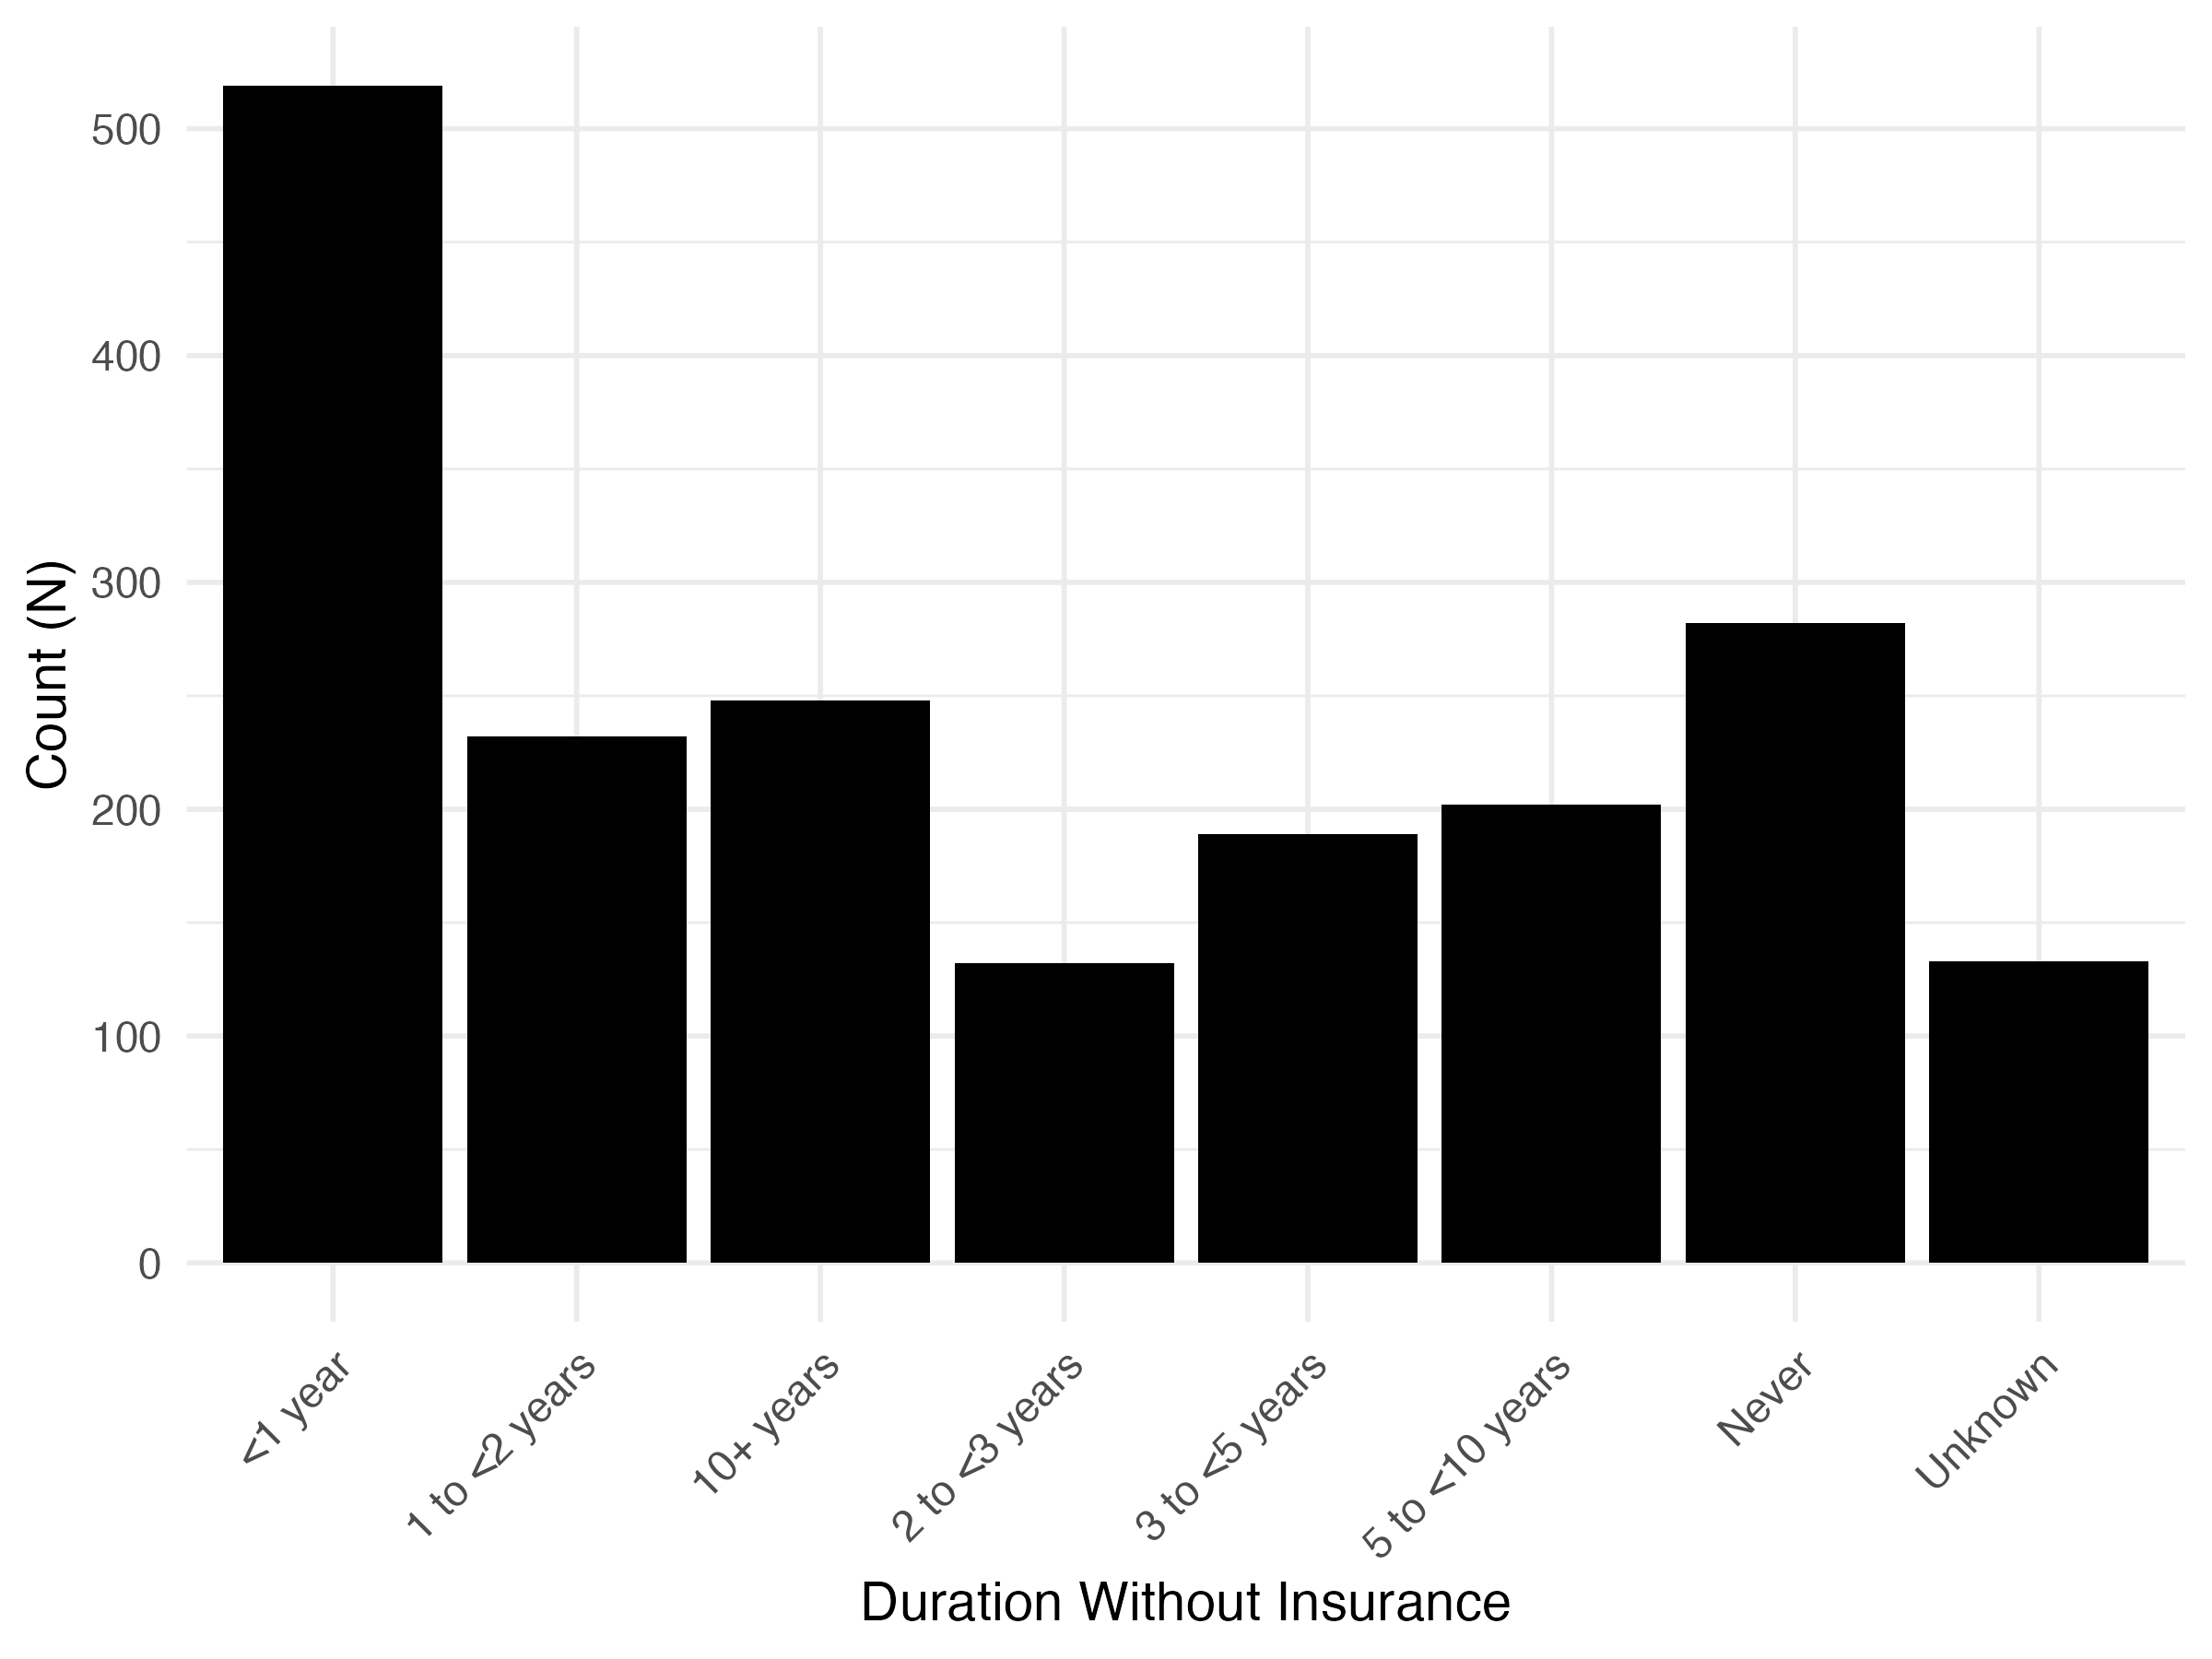
\includegraphics[width=15cm]{figures/duration_no_insurance.png}
  \caption{Distribution of duration without insurance.}
\end{figure}

% Line graph of duration without insurance by reason
\begin{figure}[H]
  \centering
  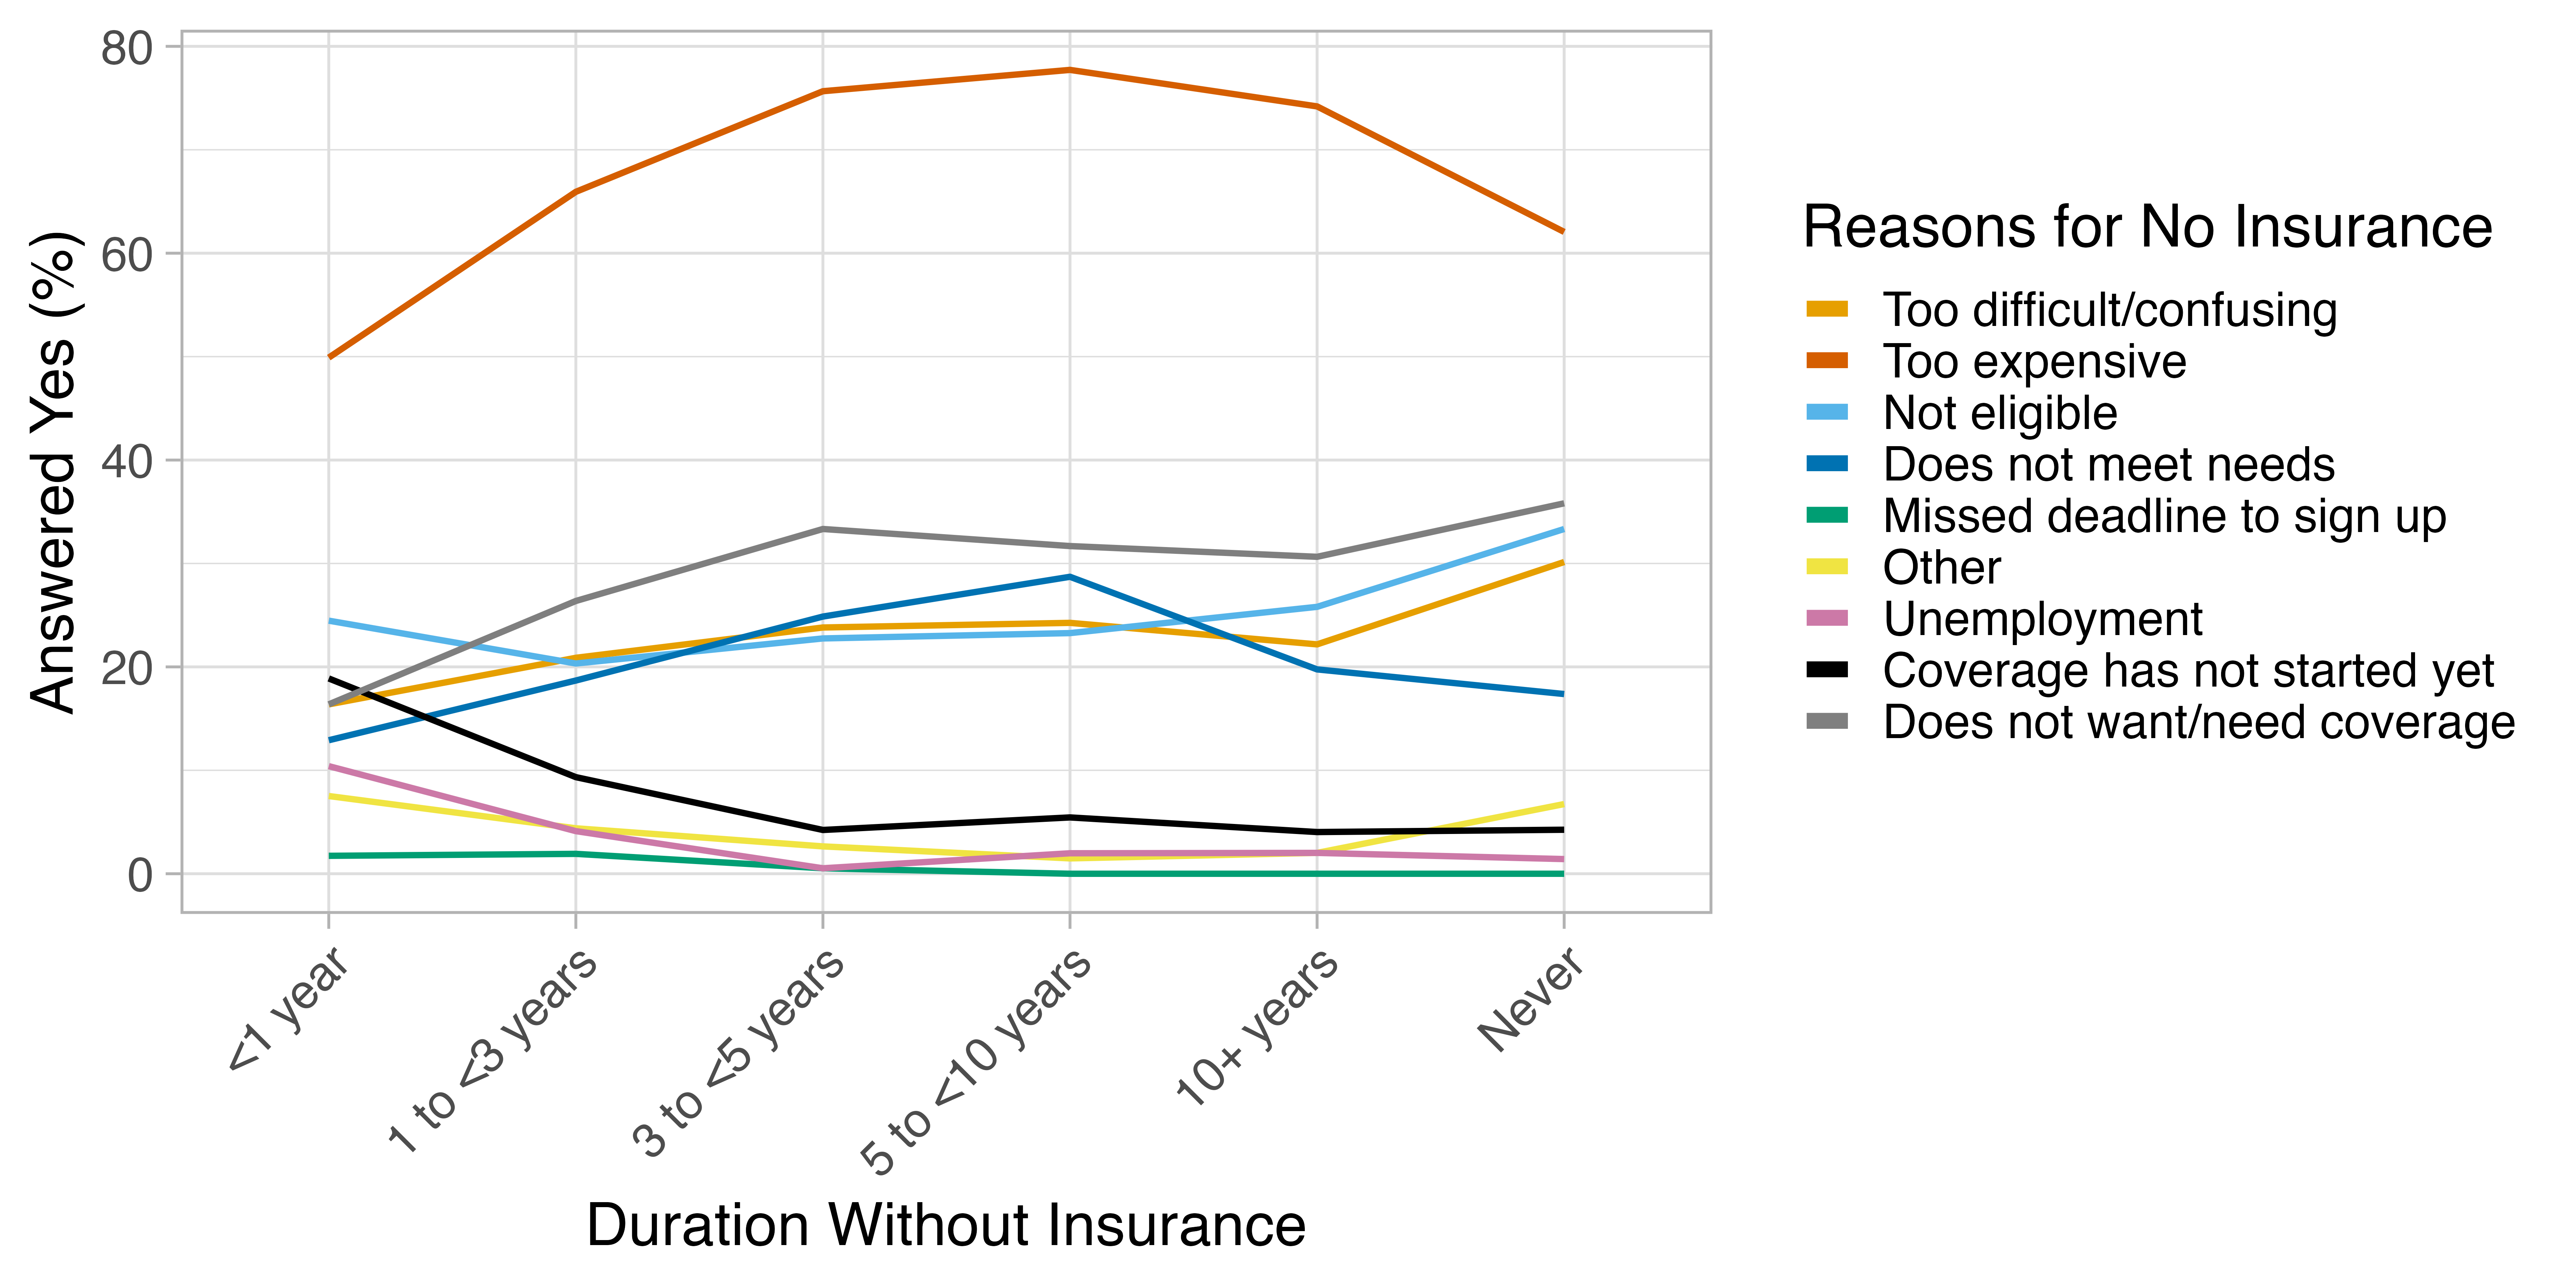
\includegraphics[width=18cm]{figures/duration_no_insurance_by_reason.png}
  \caption{Line graph of duration without insurance for each reason.}
\end{figure}


%%%%%%%%%%%%%%%%
%% DISCUSSION %%
%%%%%%%%%%%%%%%%
\newpage
\section{Discussion}


%%%%%%%%%%%%%%%%
%% REFERENCES %%
%%%%%%%%%%%%%%%%
\newpage

\printbibliography

\end{document}